\newpage

\chapter{Infrastruktur}

\section{Server}

Für die Helin Applikation steht ein Server bereit. Wie in der Abbildung \ref{fig:communication-architecture-overview} dargestellt, wird dieser sowohl für das Testing auch als Produktionsserver verwendet. 
Auf dem Server läuft PostgreSQL mit PostGIS, welche verwendet wird, um die Route zu berechnen. Daneben ist auch auf RabbitMQ eingerichtet und eine Instanz der Helin Server Applikation installiert. 
Um die Tests automatisch auszuführen wird TeamCity verwendet. Der Grund warum Test und Produktionsserver auf derselben Maschine sind, liegt daran, dass es keinen grossen Mehrnutzen für das Projekt bringen würde, falls diese getrennt sind.

Neben dem Sever werden auch zwei Android Geräte mit einer eigenen App Deployt. Beide kommunizieren primär mit der RabbitMQ Instanz auf dem Server.


\begin{figure}[h]
	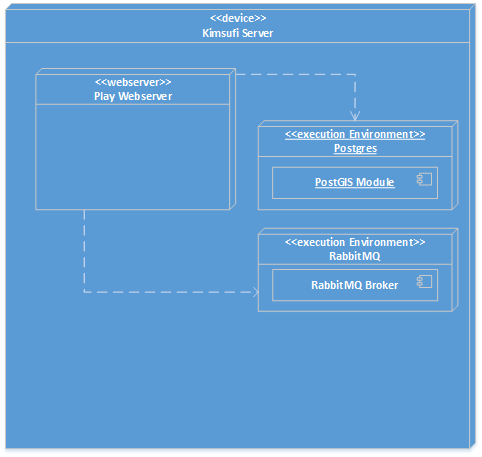
\includegraphics[width=1.0\textwidth]{images/DeploymentDiagram.png}
	\caption{Deployment Diagram}
	\label{fig:deployment-diagram}
\end{figure}


